\section{Kode}
Her vil vi forklare hvordan vi har grebet selve koden an.
\subsection{Struktur og pakker}
Ligesom i de to foregående projekter, er programmet skrevet med fokus på at overholde \textbf{BCE}-modellen. Kort fortalt betyder det for opdelingen i pakker, at alle klasser er inddelt i pakker efter deres type ift. \textbf{BCE}. For en mere uddybende beskrivelse henvises til det tilsvarende afsnit i \cite{19del1} og \cite{19del2} rapporterne.
\subsection{Genanvendelse af kode og opbygning}
På baggrund af hensigtsmæssigt og godt design i \cite{19del1} og \cite{19del2} projekterne, har det været muligt at genbruge store dele af koden. Således er klasserne \texttt{Die} og \texttt{DieCup} i praksis identiske med de tilsvarende klasser fra de tidligere projekter, ligesom den generelle opbygning af systemet også ligner meget.

På samme måde er det grundlæggende princip bag \texttt{TUI} og \texttt{Graphic} klasserne også identisk med 19del2 – klasserne har ikke behov for at bære data, og de forskellige metoder i klasserne interagerer ikke med hinanden gennem felter eller lign, og kan derfor med fordel være statiske. For en mere dybdegående forklaring henvises til kodeafsnittet i 19del2.

\subsection{Bemærkelsesværdige løsninger}
Systemet er på nuværende tidspunkt så omfattende, at det ikke giver mening at gennemgå alle overvejelser bag implementeringen af alle klasser. I stedet uddrages specielt bemærkelsesværdige dele af koden, og forklares herunder, for at give en bedre forståelse af systemets virkemåde, uden at gennemgå alt. Beskrivelserne er opdelt efter hvilke klasser de er implementeret i.
\subsubsection{TUI}
Noget af det første der sker, når dette spil startes, er at brugeren anmodes om at indtaste antallet af spillere. Antallet af spillere må ifølge opgavebeskrivelsen ikke være større end 6, og spillet giver ikke meget mening, hvis det er mindre end 2. Med andre ord skal der specifikt indtastes et tal mellem 2 og 6. Dette er en ny udfordring ift. de tidligere opgaver, hvor der blot blev gemt en hel streng. Foruden at teste, at det indtastede tal er i det krævede interval, ønskede vi også at lave systemet robust, og sikre at f.eks. bogstaver eller specialtegn indtastet på dette tidspunkt, ikke kunne få systemet til at gå ned. Dette ses i figur \vref{fig:kode1}.
\begin{figure}[!ht]
\centering
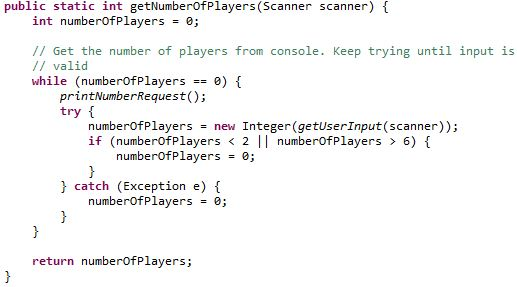
\includegraphics[width=0.8\textwidth]{kode1.jpg}
\caption[<Text for the list of figures>]{Antal spillere}
\label{fig:kode1} 
\end{figure}
Tjekket og sikringen mod karakterer som ikke er tal, sker i \texttt{TUI}, inden det sendes videre til controlleren. Antallet af spillere sættes indledningsvist til 0, og forespørgslen kører så i en løkke, som kun brydes når antallet af spillere bliver sat til noget der er forskelligt fra 0. Det input der hentes fra konsollen er som udgangspunkt en streng, og skal derfor konverteres før det kan bruges som en talværdi. Denne konvertering vil kaste en Exception, hvis der gives et input, der ikke umiddelbart giver mening som tal-værdi – f.eks. et bogstav. Det smarte er så, at denne Exception kan fanges, og kode kan udføres til at ”reparere” den fejl, som har forårsaget den. I vores tilfælde sætter vi bare værdien for antal af spillere tilbage til 0, fordi det betyder at løkken kører igen, så brugeren bliver spurgt efter et nyt input.
Ligeledes hvis der gives et input, som succesfuldt kan konverteres til en talværdi, tjekkes der om tallet er mellem 2 og 6 – hvis ikke det er det, sættes værdien tilbage til 0, og løkken kører igen. Så snart løkken brydes, returnerer metoden.

\subsubsection{GameBoard}
Ligesom ved et fysisk spil, indeholder dette system en spilleplade \texttt{GameBoard}, som er bygget op af felter af forskellig type. Disse felter er bygget i et system med arv, som beskrevet senere i dette afsnit, og dette giver en stor fordel for datastrukturen i \texttt{GameBoard}. Fordi alle de forskellige felttyper \texttt{Territory, LaborCamp, Fleet, Tax og Refuge} nedarver fra Field, kan der laves en enkelt liste (array) af felter, af typen \texttt{Field}, som kan indeholde alle de forskellige felter, selvom der er tale om forskellige typer objekter, med forskellige implementeringer af metoder mm. Koden ses i figur \vref{fig:kode2}.
\begin{figure}[!ht]
\centering
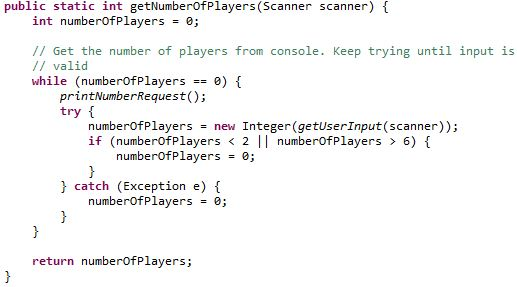
\includegraphics[width=0.8\textwidth]{kode1.jpg}
\caption[<Text for the list of figures>]{Antal spillere}
\label{fig:kode2} 
\end{figure}
\subsubsection{Field} 
Som nævnt tidligere, er felterne bygget op med at system af arv. Alle felterne nedarver fra \texttt{Field}, som indeholder de ting der er fælles for alle felter. I realiteten er det ikke ret meget der er det samme for alle felter – der er forskellige muligheder ift. køb, der er forskellige konsekvenser (få penge, miste penge), og selv de felter der har den samme konsekvens – at man skal betale til andre – har forskellige måde at beregne beløbet på.

Alle felter har dog et navn, og alle felter har mulighed for at man kan lande på dem. Derfor indeholder \texttt{Field} et felt til navn, og en abstrakt metode – \texttt{landOnField} – der betyder at alle klasser som arver fra \texttt{Field}, skal ”love” at de implementerer \texttt{landOnField}. De forskellige underklasser kan så have forskellige implementeringer af \texttt{landOnField}, så længe typen af parametre og returværdi er de samme.


To typer felter – \texttt{Tax} og \texttt{Refuge} – nedarver direkte fra \texttt{Field}, men de resterende 3 felttyper nedarver i stedet fra \texttt{Ownable}, som så igen nedarver fra \texttt{Field}. Dette skyldes, at disse 3 felter – \texttt{Territory, LaborCamp} og \texttt{Fleet} – kan købes. Dette er en funktionalitet, som grundlæggende vil virke ens for alle tre typer felter – der skal være et pegepind til en ejer, der skal være en måde at købe feltet osv.
Desuden vil den grundlæggende procedure, når der landes på feltet, også være ens – der skal tjekkes om der er nogen der ejer feltet, og hvis der er, skal der betales leje til ejeren. Hvordan lejen udregnes, er forskellige for de forskellige typer at felter, men den overordnede procedure er ens. Derfor er \texttt{landOnField}-metoden, der som bekendt skal implementeres, når klasserne arver fra \texttt{Field}, implementeret i \texttt{Ownable}. Metoden i \texttt{Ownable} kalder så \texttt{getRent-metoden}, der har forskellig implementering i hver af underklasserne.
\subsubsection{Fleet}
Af de underklasser, hvor der skal udregnes leje, er \texttt{Fleet} en af de mere interessante. Lejen for \texttt{Fleet} afhænger nemlig af hvor mange andre \texttt{Fleet}-felter ejeren af det felt der landes på, har. Det betyder, at det \texttt{Fleet}-felt der er landet på, er nødt til at kende ejeren af de øvrige \texttt{Fleet}-felter, for at kunne udregne lejen.
I praksis implementeres det ved, at et \texttt{Fleet} felt-objekt tager den spilleplade \texttt{GameBoard} det oprettes i, med som parameter, når det oprettes. Således har \texttt{Fleet}-feltet mulighed for at gå ud og se på andre felter på den samme spilleplade.

Dernæst er problematikken blot, at de objekter på spillepladen, som dette objekt nu har adgang til, er af typen \texttt{Field}. Overklassen \texttt{Field} indeholder ikke en ejer, så før ejeren af feltet kan findes, må det konverteres til \texttt{Ownable}. Herefter er det blot en simpel løkke, som tjekker ejeren på hvert \texttt{Fleet}-felt, og summerer op. Når antallet af \texttt{Fleet}s er fundet, kan lejen simpelt findes med en switch-sætning.
\subsubsection{LaborCamp}
På samme måde som \texttt{Fleet}, bruges antallet af ejede felter af samme type også til beregningen af lejen ved \texttt{LaborCamp}. Fremgangsmåden til at finde antallet af ejede felter, er helt den samme som ved \texttt{Fleet}.
Foruden antallet af ejede \texttt{LaborCamps}, indgår også et terningslag i beregningen af lejen – det betyder at \texttt{LaborCamp} er nødt til at have kendskab til \texttt{DieCup}, for at kunne få værdien af et terningslag. Imidlertid befinder\texttt{DieCup} sig på spillepladen \texttt{GameBoard}, så i kraft af at \texttt{LaborCamp} allerede har \texttt{GameBoard} med som argument, for at kunne kigge på andre felter, har den også let adgang til \texttt{DieCup}.
\subsubsection{Ownable}
Som nævnt tidligere i afsnittet, er der 3 felttyper som kan købes. Nå en spiller køber et felt, skal der trækkes nogle penge fra spillerens konto, og \texttt{owner}-pegepinden i feltet skal sættes til at pege på spillerens objekt. Før dette sker, skal der imidlertid have været præsenteret et valg for spilleren, om hvorvidt denne ønsker at købe feltet eller ej, og lige netop dette viser sig at være den mest krævende del at implementere af denne funktionalitet.


Ideen med hele opbygningen af systemet efter \textbf{BCE}-modellen er nemlig, at elementer fra entitets-laget aldrig har direkte adgang til elementer fra brugergrænseflade-laget. Men for at kunne præsentere valget om køb for spilleren, er feltet nødt til at kalde \texttt{TUI}’en, for at printe på skærmen og tage input fra konsollen – og vil netop give det føromtalte uønskede kendskab fra brugergrænsefladen til en entitet. Alternativt kunne man måske forstille sig, at feltet så havde kendskab til controlleren, og så kunne kalde TUI’en den vej igennem, men det vil også bryde mønsteret – ideen er jo at det er controlleren der skal kontrollere programmet, og kalde metoder i entiteter og brugergrænsefladen.


Uanset hvordan det drejes, er der ikke rigtigt en perfekt løsning på denne problemstilling – i hvert fald ikke uden at der skal ændres på de metoder, som er givet i opgavebeskrivelsen, der som udgangspunkt ikke må ændres. Med andre ord handler det nok om at finde den mindst dårlige løsning.


I vores projekt vælger vi at udnytte, at både felterne og controlleren har kendskab til spillerens objekt. I stedet for at kalde en metode, når en bruger lande på et felt der kan købes, sættes således et ”flag” i spillerens objekt \texttt{isOnBuyableField = true}. Når der så returneres til controlleren, kan der tjekkes på om spilleren står på et felt der kan købes, og selve købet foretages i controlleren, som jo har kendskab til både \texttt{TUI} og felterne.
\subsubsection{Tax}
Der er to typer af \texttt{Tax} – den simple, hvor der blot betales et fast beløb, og den mere avancerede, hvor der kan vælges mellem et fast beløb og en procentdel af spillerens formue. Sidstnævnte er interessant, dels fordi den er nødt til at kende ejeren af alle andre felter, for at kunne beregne spillerens formue, dels fordi den skal spørge spilleren hvilken mulighed der foretrækkes.

At beregne formuen er i store træk implementeret på samme måde som \texttt{Fleet} og \texttt{LaborCamp} – feltet tager \texttt{GameBoard} med som parameter, og kan så få fat i ejeren af de andre felter. Her summers så ikke op på antal, men på pris.


At spørge brugeren, giver til gengæld samme problematik som omtalt ved køb af felter i \texttt{Ownable} – en entitet er nødt til at ”snakke” med brugergrænsefladen. Det kunne løses på samme måde som ved køb af felter, ved at bruge spillerens objekt til at gemme et ”flag”, men forskellen er, at både det faste \texttt{Tax}-beløb og det udregnede procentvise \texttt{Tax}-beløb er nødt til at med ud til controlleren, for at der kan opkræves korrekt. Det betyder dels, at der, foruden ”flaget”, også skal gemmes to talværdier i spillerens objekt, og dels at man effektivt vil have flyttet hele logikken fra Tax ud i controlleren.
I praksis vil den løsning ganske vist løse opgaven og give pæne diagrammer, hvor der ikke er nogen synlig kobling mellem \texttt{Tax} og \texttt{TUI} – men reelt giver det en skjult kobling, som måske i virkeligheden er højere end den ville være, hvis \texttt{Tax} bare havde kendskab direkte til \texttt{TUI}, og som under alle omstændigheder er langt sværere at gennemskue.


Derfor vælger vi at lade \texttt{Tax} have kendskab til \texttt{TUI}, men knytter hertil samtidigt en klar bemærkning om, at dette er et af de steder hvor systemet kan forbedres.
\subsubsection{Game}
Strukturen og ideen i \texttt{Game}-controlleren er stadig helt den samme som i de tidligere projekter. En af de største forskelle i controlleren, er muligheden for mere end 2 spillere, og måske endnu vigtigere, det faktum at der ikke bare er en spiller som vinder – der er spillere som taber løbende, og som så skal udgå af spillet. Det betyder nemlig, at der ikke blot kan laves en simpel valgsætning, som afgør om en spiller har vundet – i stedet må der tælles hvor mange spillere der er tilbage, hver gang en spiller er udgået.
\newpage